\section{Evaluating the Framework in Practical Applications}

Since the framework we are developing is intended for real-world projects, this validation aims to demonstrate its full functionality using practical, real-world scenarios. The objective is to show how the framework operates in realistic projects, ensuring its effectiveness in handling real software systems. As discussed earlier, each scenario represents common use cases that can arise during project maintenance. Since reverse engineering is mainly used to break down complex software into smaller, manageable components, it becomes a valuable tool in the maintenance and evolution of software projects. By dissecting an existing system, it helps developers understand its structure, dependencies, and functionality, making future modifications and improvements more manageable.

It is important to note that evaluating the framework does not solely rely on the current probes' output, as the overall results can vary depending on the probes used for each project. Instead, the validation focuses on whether the framework as a whole functions as expected, regardless of the specific probes implemented. To establish its working, the real-world scenarios defined in this report must demonstrate that the framework successfully processes and analyzes software systems as intended. In short, the goal is to provide a structured and functional approach to reverse engineering, ensuring that it can be effectively applied in practical scenarios.

% Once the graph data is uploaded to the SST server and stored in Neo4j, it is time to view this data in the visualizer. In this project, we are using Neo4j desktop application and Tableau to view the data. Once

% \begin{figure}[H]
%     \centering
%     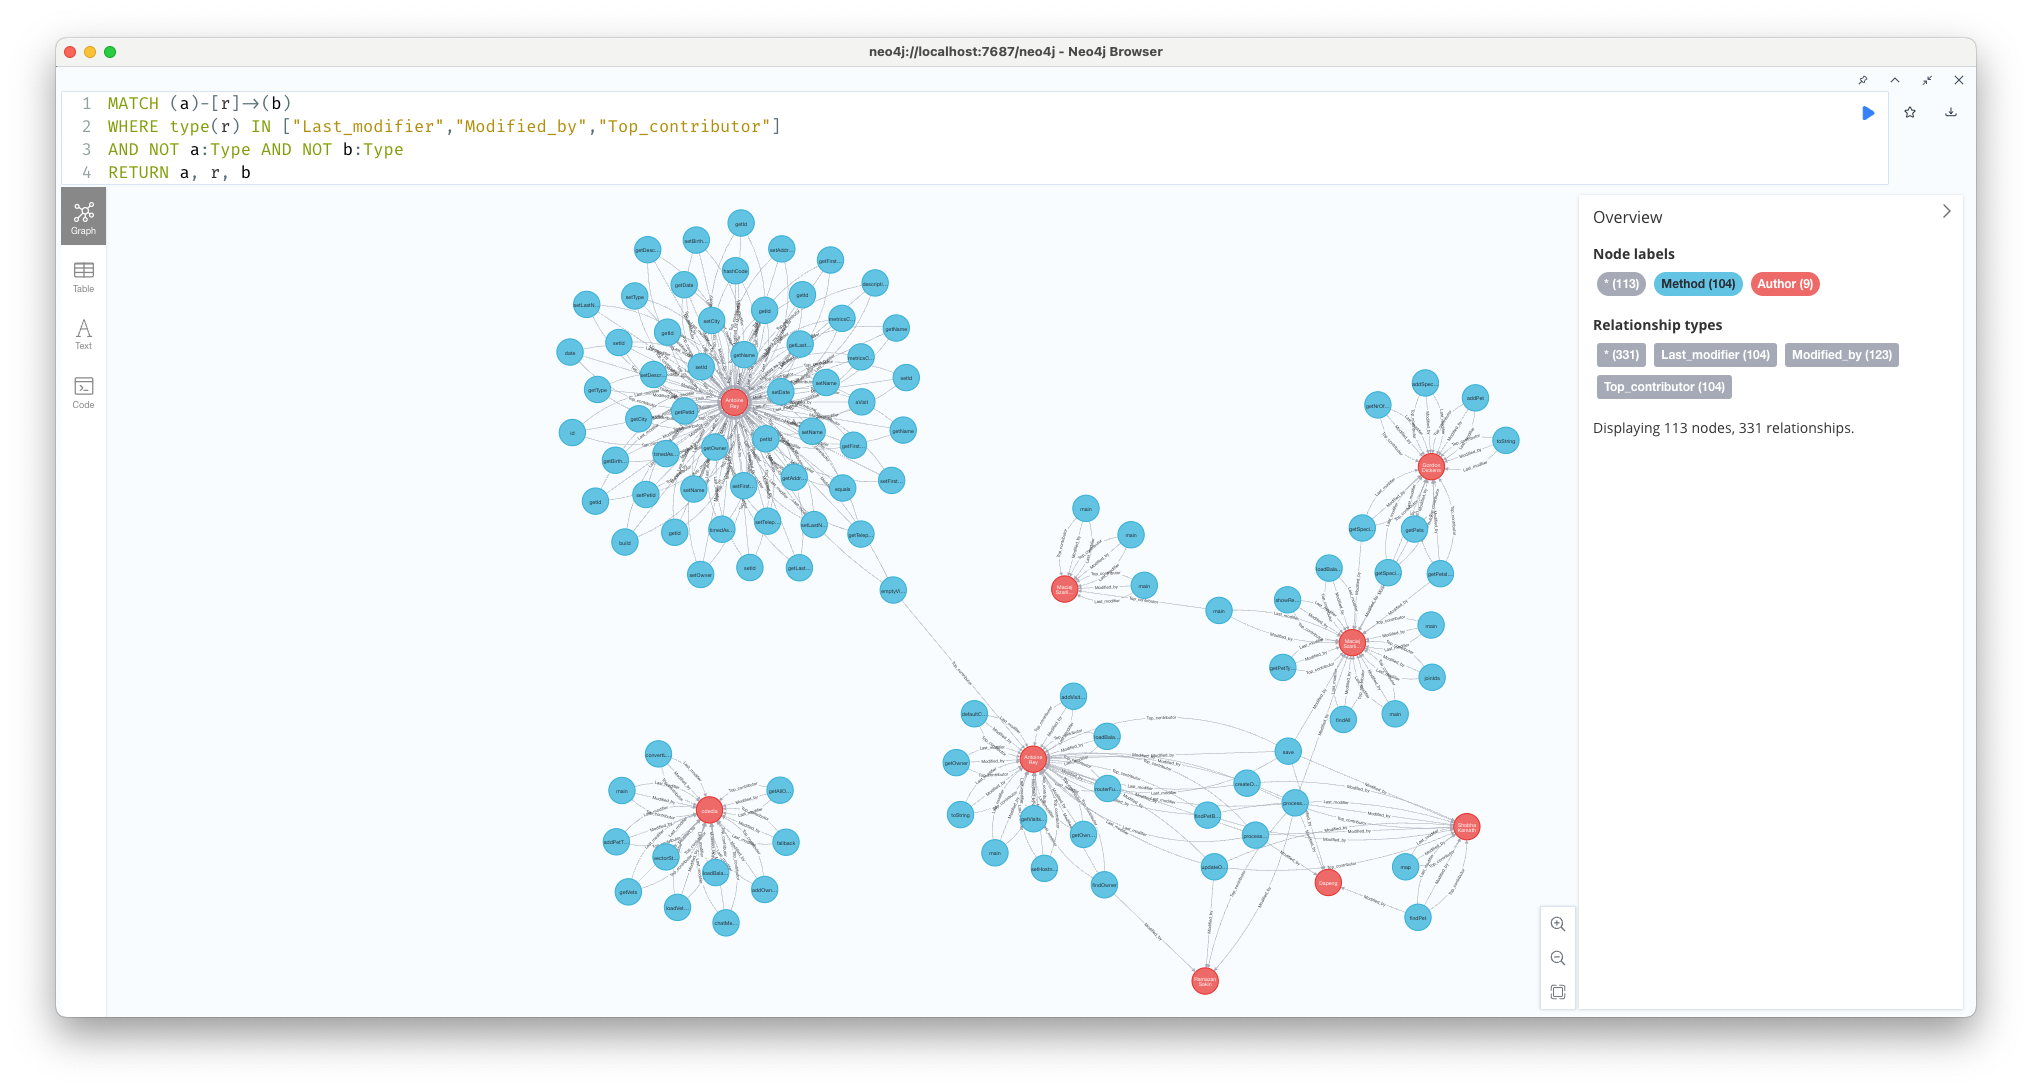
\includegraphics[width=1\textwidth]{figures/scenario_1_2_3.png}
%     \caption{Neo4j Browser showing relation between nodes for scenario 1,2 and 3}
%     \label{fig:scenerio_1_2_3_overview}
% \end{figure}

% In this section, we will demonstrate the output of the first three scenarios, most recent, all and top contributors of methods. We can show the nodes relation graph diagram using Neo4j browser. Since all three probes are related to methods and authors, we can output nodes showing methods and authors, and edges showing the relation of each node with the other one. We can use Neo4j Cypher queries\footnote{\url{https://neo4j.com/docs/cypher-manual/current/queries/}} to filter out the required data.

% \begin{figure}[H]
%     \centering
%     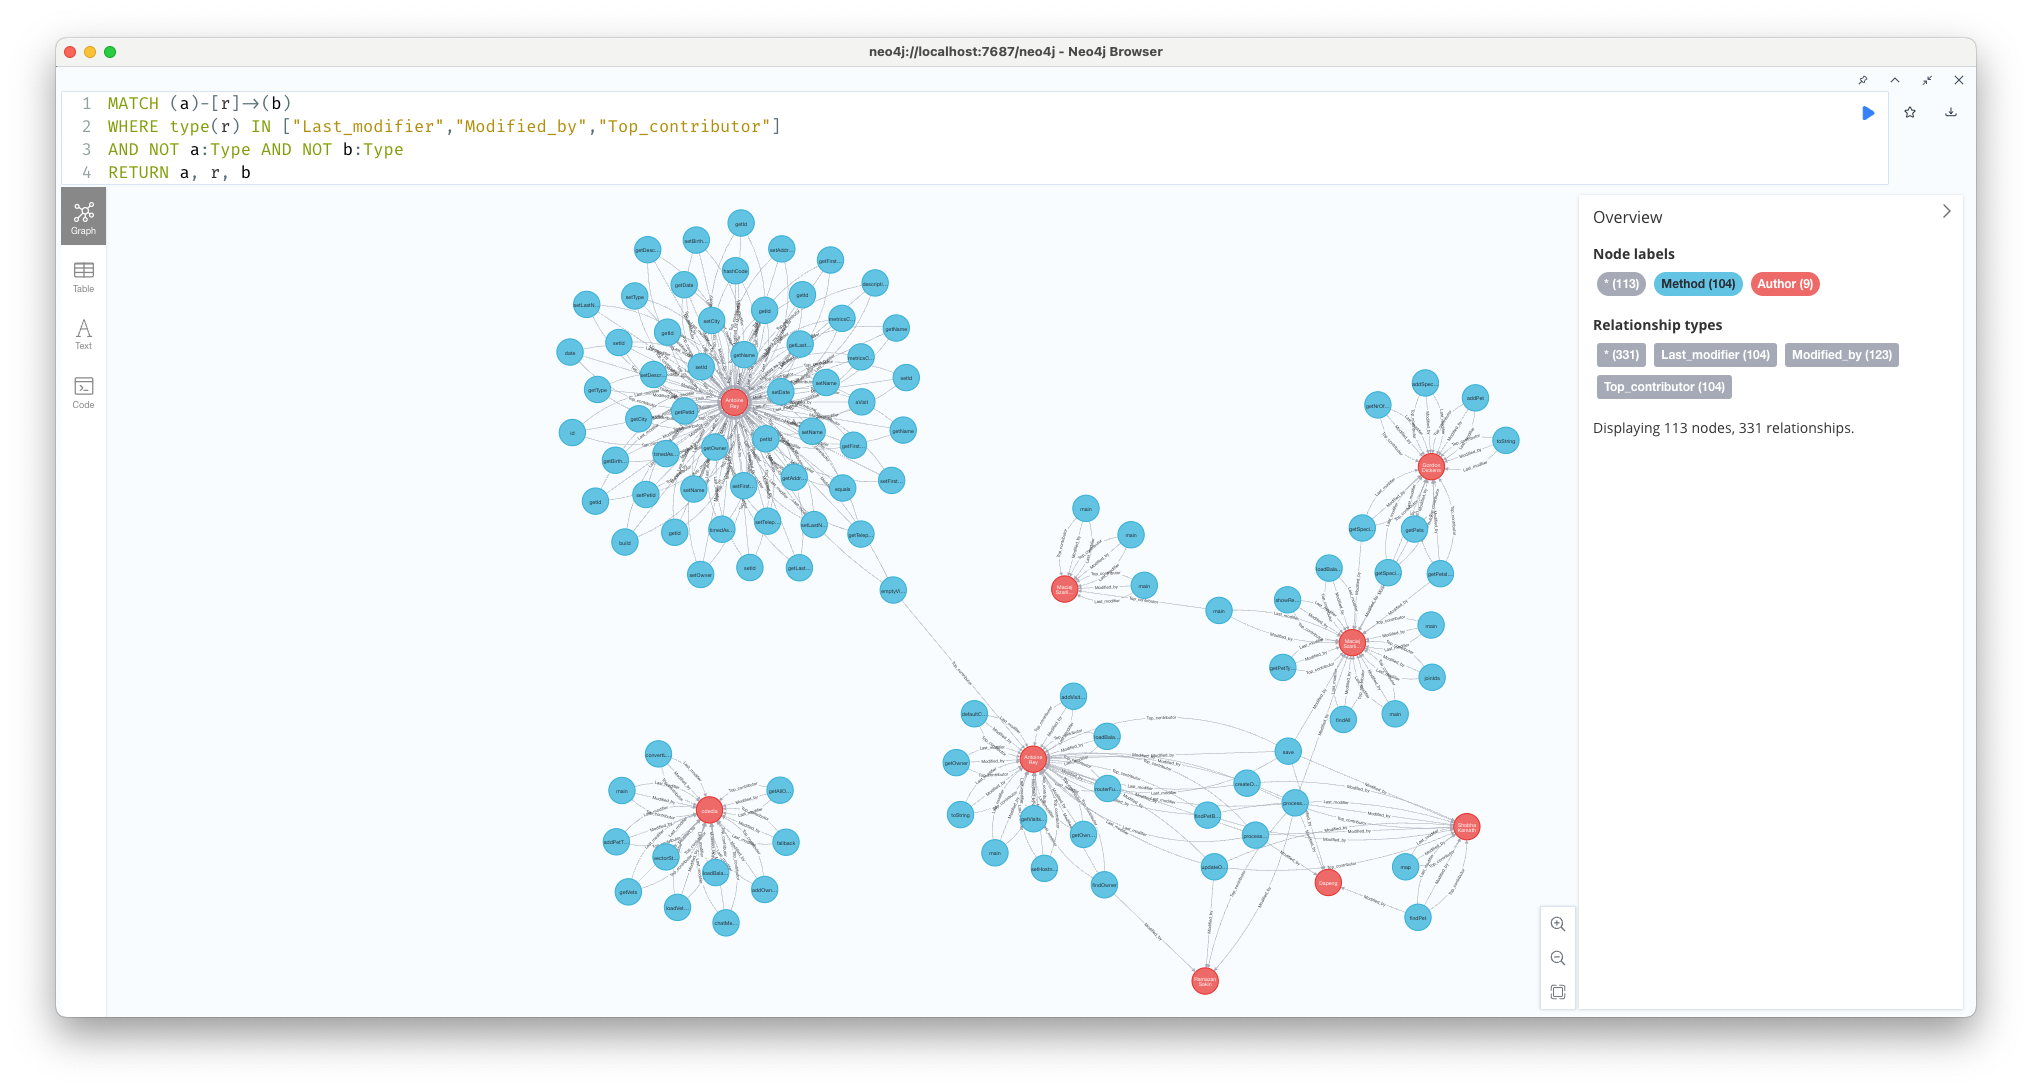
\includegraphics[width=1\textwidth]{figures/scenario_1_2_3.png}
%     \caption{Neo4j Browser showing relation between nodes for scenario 1,2 and 3}
%     \label{fig:scenerio_1_2_3_overview}
% \end{figure}

% For better explanation, we can pick out one of the methods to have a close look at it.